\documentclass[]{article}

\usepackage{acro}
\usepackage{listings}
\usepackage{cleveref}
\usepackage{xcolor}
\usepackage{graphicx}
\usepackage[style=numeric]{biblatex}
\addbibresource{./literature.bib}


\definecolor{superlightgray}{rgb}{0.9, 0.9, 0.9} 

\lstset{
	numbers=left,
	stepnumber=1, 
	tabsize=4,
	backgroundcolor=\color{superlightgray},
	basicstyle=\footnotesize,
	breaklines=false,
	rulecolor=\color{black},
	commentstyle=\color{blue},
	keywordstyle=\color{red},
	numberstyle=\scriptsize\color{black},
	stringstyle=\color{purple},
	columns=fullflexible
}
\DeclareAcronym{msaa}{
	short = MSAA,
	long = {Multi Sampling Anti Aliasing}
}

\DeclareAcronym{fov}{
	short = FOV,
	long = {Field of View}
}

\DeclareAcronym{ior}{
	short = IOR,
	long = {Index Of Reflection}
}

\graphicspath{{../images_report/}}

\title{Ray-tracing based renderer from scratch in Python}
\author{Jörn Lasse Vaupel}
\date{\today}

\begin{document}
	
	\maketitle
	\newpage
	\tableofcontents
	
	\begin{abstract}
		
	\end{abstract}

	\newpage
	
	\section{Introduction}
	\label{sec:intro}
	This report summarizes the process of implementing a ray-tracing based renderer from scratch following the introduction from Peter Shirley’s Ray Tracing in One Weekend  \cite{Shirley2020RTW1} and its continuation Ray Tracing: The Next Week \cite{Shirley2020RTW2}. While Shirley used C++ as a high performance and efficiency programming language, the following implementation is written in Python.  Even if the rendering times may be longer, Python’s readability and easiness helps focusing on the basic concepts of ray-tracing based rendering. In addition, efficiency might be higher if the advantages of Python libraries like \emph{NumPy} would be used more strictly, but the focus of the implementation is on understanding, not on efficiency. All in all, some functionalities are just easier to implement in Python than in C++.
	\\
	In the working process many different test images were rendered. In order to meet all the requirements for the final result and generate a uniformly growing scene, the implementation was completed before rendering the final images taking into account a backwards compatibility. Therefore, all final images can be generated by using the same structure: a scene containing one or several cameras and some spheres. Only the single-colored image is generated differently due to the gamma correction. This shows some design decisions in the implementation like a horizontal \ac{fov} or gamma correction, can lead to slightly different results than those, that were possible in previous stages of implementation. This is no big deal but should be mentioned.
	
	\section{First rendering loop}
	Just with the beginning the first example of understanding against efficiency occurs. In order to speed up rendering and to limit the amount of file accesses, the rendered image is saved in an image array maintained by an \emph{Image} class before saved in a .ppm file. The rendering loop requires a double for loop. To avoid generating the file from scratch within another double for loop, it’s possible to use Python libraries like \emph{Pillow} to directly write a .ppm file. But to enable a deeper understanding of the structure of the file format while utilizing the advantages of Python libraries, a custom approach based on \emph{NumPy} is used (the double for loop approach is also shown but not used).
	\\
	The code from \emph{scene1.py} in \cref{lst:first_render_loop} shows the basic use of the \emph{Image} class and the render loop which generates the image in \cref{fig:image1}. The render loop will be later handled by the \emph{Camera} class.
	
	\begin{lstlisting}[caption={Example for a basic render loop}, language=Python, label=lst:first_render_loop]
image = Image(1920, 1080)
for y in range(image.height)[::-1]:
	for x in range(image.width):
		image.image_list[y, x] = Vector(128, 64, 255).to_int_array()

image.save_image("../images/image1.ppm")
	\end{lstlisting}

	\begin{figure}[h]
		\centering
		
\includegraphics[width=0.9\linewidth]{image1}
		\caption{Singe-colored image generated by first render loop}
		\label{fig:image1}
	\end{figure}

	\section{Camera}
	\label{sec:camera}
	The implementation of the camera in the \emph{Camera} class largely follows the tutorial in \cite{Shirley2020RTW1}. In general, it’s necessary to define a large set of algebraic methods within the \emph{Vector} and \emph{Ray} class. Referring the \emph{Vector} class, it’s important to mention that the default operators (e.g. \textbf{+} and \textbf{-}) are overloaded and especially the meaning of \textbf{*} operator depends on the second operand. If it’s a float the operation defines a scalar multiplication, if it’s a vector the result is the dot product of both vectors.
	\\
	A small addition to the concept in \cite{Shirley2020RTW1} used in this implementation is the idea that every object within a 3D scene has a position (and a rotation) and can therefore be described as an object of a common class: the \emph{Transform} class. This does not grant any advantages now but makes the implementation of new 3D objects like spheres (or maybe a collection of planes in future) easier.
	\\
	The main difference between this implementation and the approach in \cite{Shirley2020RTW1} is a design decision regarding the rendering loop and the sent out rays. To get such a ray, which can collide with objects later, the \emph{get\textunderscore ray(x, y, antialiasing)} method was implemented. While the tutorial uses the image plane coordinates for x and y, this implementation considers the pixel coordinates as \emph{x} and \emph{y} and transforms them into world space (image plane) coordinates in the method itself. This approach helps understanding, that for each image pixel one ray is generated. In case of antialiasing multiple rays for each pixel are sent out (\emph{antialiasing} parameter) as explained more detailed in \cref{sec:antialiasing}. \Cref{lst:getray} shows the code of the \emph{get\textunderscore ray(x, y, antialiasing)} method.
	\\
	The resulting image generated with \emph{scene2.py} is shown in \cref{fig:image2}. Because of the lag of backwards compatibility described in \cref{sec:intro} or - to be more precisely - due to personal favor, the \ac{fov} is slightly different in all rendered images (more details in \cref{sec:fov}). 

	\begin{figure}[h]
		\centering
		
\includegraphics[width=0.9\linewidth]{image2}
		\caption{Gradient image generated by camera (empty 3D scene)}
		\label{fig:image2}
	\end{figure}

	\section{Spheres}
	Just like the implementation of the camera the implementation of spheres within the \emph{Sphere} class was straight forward understanding the concepts from \cite{Shirley2020RTW1} and transfer them to Python. Key feature is the \emph{hit(ray, t\textunderscore min, t\textunderscore max)} method every 3D object which can interact with camera rays must have. Therefore the class \emph{RenderObject} is defined which inherits from \emph{Transform} class and provides an abstract method \emph{hit(ray, t\textunderscore min, t\textunderscore max)}. That method later has to be implemented by the sub classes of \emph{RenderObject} like \emph{Sphere}.
	\\
	In case of the \emph{Sphere} class the intersection of ray and sphere is calculated using an optimized equation based on the radius and position of the sphere. Because most of the times two intersections will be detected for each ray, only the closer point is used. The method also returns the normal in the intersection point and flips it if the ray was emitted from within the sphere. On this place the implementation varies from the approach in \cite{Shirley2020RTW1}. The ray is outside the sphere if the dot product of the ray’s direction and the normal in the intersection point is greater than or equal to 0 (if both are orthogonal it’s still outside), while there is only $<$ used in \cite{Shirley2020RTW1}. For numerical approaches this makes no big difference, because this case rarely occurs but for correctness and understanding this was changed (logical difference between Listing 17 and Listing 18 in \cite{Shirley2020RTW1}).
	\\
	The \emph{hit(ray, t\textunderscore min, t\textunderscore max)} also allows to limit the render distance by the \emph{t} parameters (close and far range) and is used by \emph{ray\textunderscore color(ray, scene, depth)} method to return color (or later material) of the sphere.
	\\
	Adding five spheres of different radius and color to a 3D scene of \emph{Scene} class (described in \cref{sec:scene}) results in a rendered image like in \cref{fig:image3}.
	
	\begin{figure}[h]
		\centering
		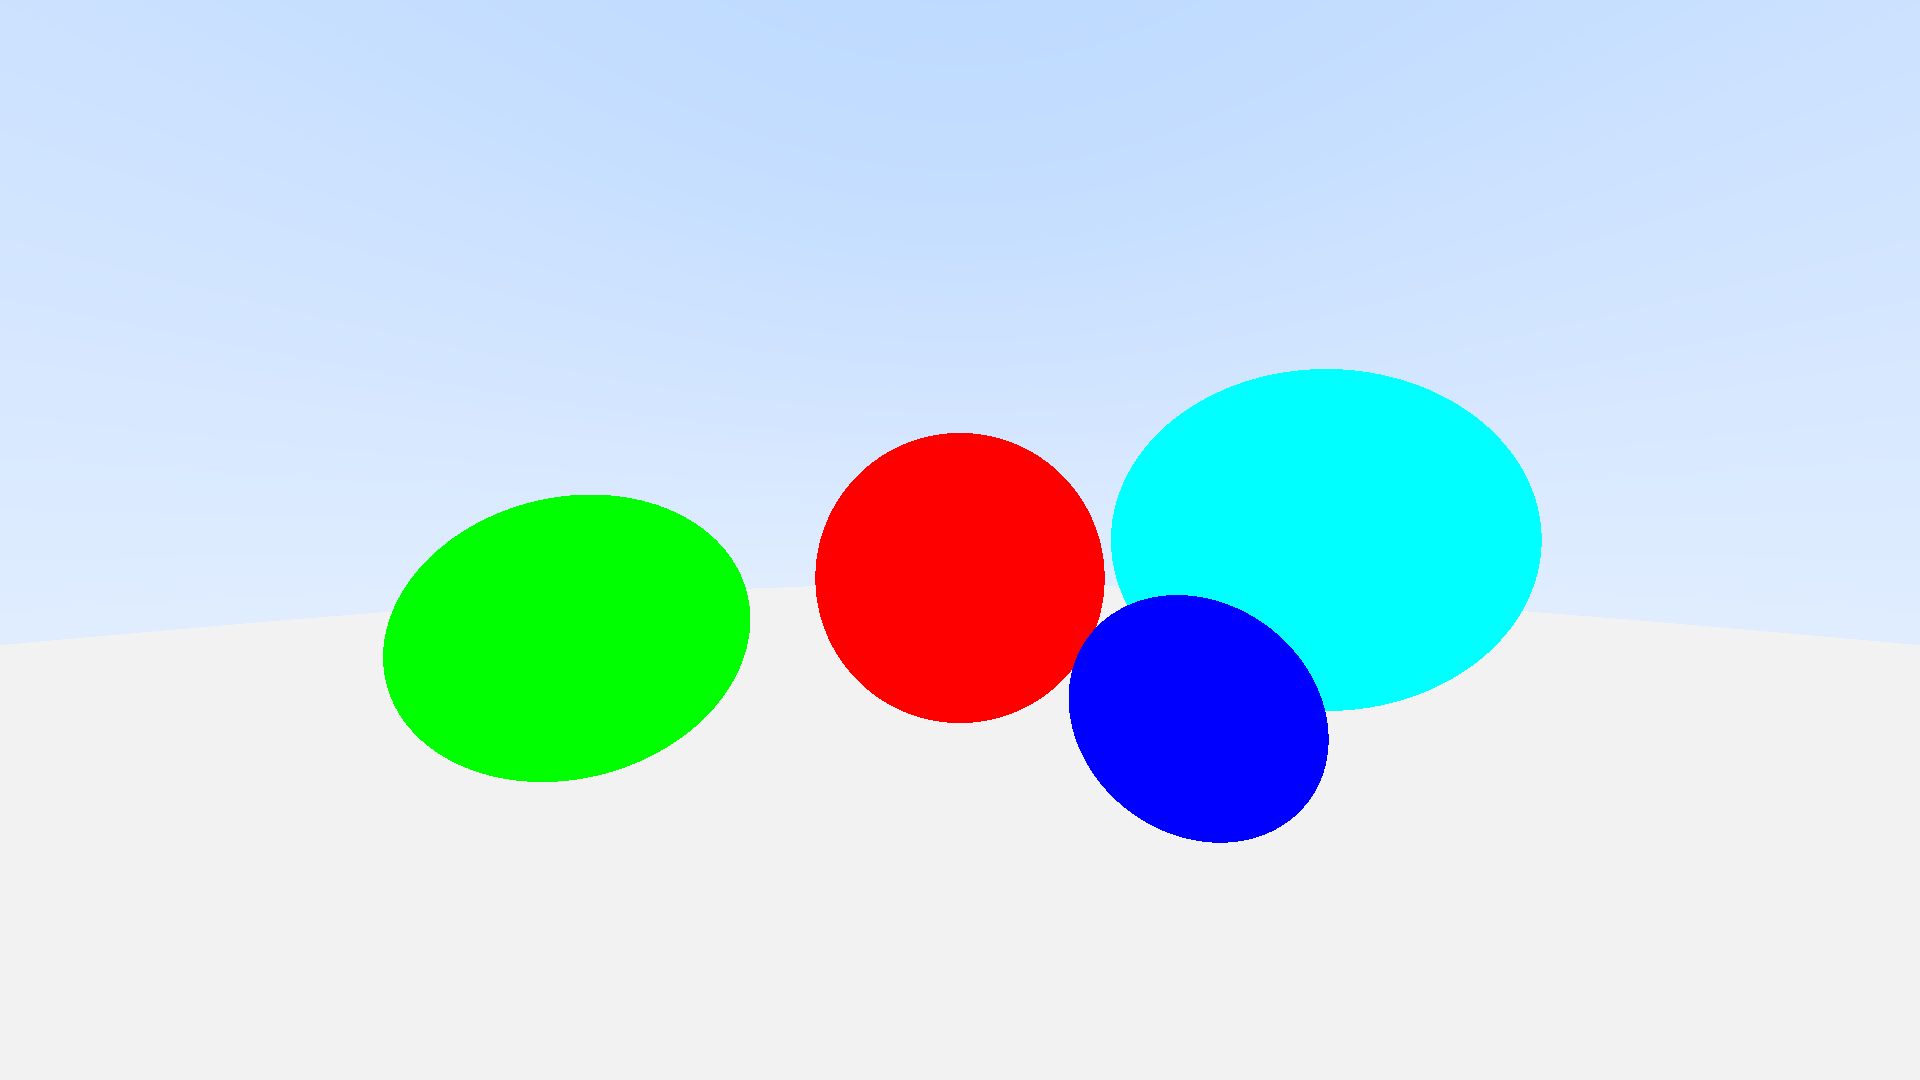
\includegraphics[width=0.9\linewidth]{image3}
		\caption{Scene of five spheres with different plain colors}
		\label{fig:image3}
	\end{figure}

	\subsection{Scene}
	\label{sec:scene}
	A 3D scene can contain a bunch of different objects which are rendered from one or more cameras. The \emph{Scene} class represents such a scene and allows to handle one or more cameras of \emph{Camera} class which render objects of \emph{RenderObject} class within the scene by calling the \emph{Scene} objects \emph{render()} method which is successively calling the cameras \emph{render()} methods. 
	\\
	This class is the interface for the user to generate the desired scene and render it within just on python file like for \emph{scene3.py} in \cref{lst:scene_example}.
	\begin{lstlisting}[caption={Example for Scene class usage from scene3.py}, language=Python, label=lst:scene_example]
from geometries import Vector
from objects import Scene, Camera, Sphere

scene = Scene("../images/image3")
# camera
main_camera = Camera(16 / 9, 1920, 1)

# spheres
s0 = Sphere(Vector(0, -1, -13), 4, color=Vector(1, 0, 0))
s1 = Sphere(Vector(-8, -2, -10), 3, color=Vector(0, 1, 0))
s2 = Sphere(Vector(4, -3, -8), 2, color=Vector(0, 0, 1))
s3 = Sphere(Vector(10, 0, -14), 5, color=Vector(0, 1, 1))
s4 = Sphere(Vector(0, -1005, -2), 1000, color=Vector(.9, .9, .9))

scene.add_render_object(s0)
scene.add_render_object(s1)
scene.add_render_object(s2)
scene.add_render_object(s3)
scene.add_render_object(s4)

scene.add_cam(main_camera)
scene.render()
	\end{lstlisting}
	
	\section{Antialiasing}
	\label{sec:antialiasing}
	Looking at the silhouettes of the spheres closely reveals some hard edges. The color of the background and the spheres can be clearly separated and do not fade into each other. Therefore, the final image seems less realistic and more pixelated. In order to get smoother transmissions antialiasing is used. In this case like in the tutorial \ac{msaa} is implemented.
	\\
	Doing this, instead of generating just on ray sent out per image pixel as in \cref{sec:camera}, multiple of those rays are generated. To obtain a small direction offset for each ray the intersection position with the image plane (ray goes through camera origin and this point) is randomly shifted.
	\\
	This random factors for \emph{x} and \emph{y} are calculated using \emph{NumPy’s random\textunderscore uniform(0, 1)} method, which returns a random value in the interval [0, 1). Without this offset the ray would go through the lower-left corner of each pixel in the image plane. This calculations are done in \cref{lst:getray}, all additional lines of code regarding lenses are explained in \cref{sec:depthoffield}.
	\\
	The color information of the intersections of those rays returned by \emph{ray\textunderscore color(ray, scene, depth)} method are summed up per pixel and later divided by the amount of samples per pixel (given to the constructor of an object of \emph{Camera} class by \emph{samples\textunderscore per\textunderscore pixel} parameter). 
	\\
	The \emph{clamp(min, max)} method implemented in the tutorial to clamp the colors between 0 and 255 (probably due to a C++ limitation or personal favor), is not used in this implementation, because all single colors are used to be between 0 and 1. The sum of all colors therefore can’t be negative nor bigger than $255\cdot  samples\textunderscore per\textunderscore pixel$. The transformation to RGB values between 0 and 255 is done in the \emph{write\textunderscore color(pixel\textunderscore color)} method together with gamma correction later on.
	\\
	Based on this implementation images with different levels of \ac{msaa} can be calculated with \emph{scene4.py} (\ac{msaa}-1 is like without antialiasing). A detailed comparison is visualized in \cref{fig:image4}. While \ac{msaa}-2 is still quite pixelated, \ac{msaa}-16 looks clearly smoother. Following images will be rendered with \ac{msaa}-64, to avoid aliasing as a source of error.
	
	\begin{figure}[h]
		\centering
		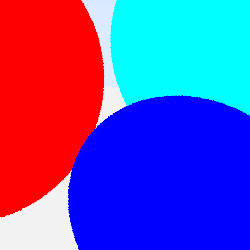
\includegraphics[width=0.45\linewidth]{image4-2-zoom}
		
\includegraphics[width=0.45\linewidth]{image4-5-zoom}
		\caption{Cropped images of spheres with \ac{msaa}-2 (left) and \ac{msaa}-16 (right)}
		\label{fig:image4}
	\end{figure}
	
	\section{Materials}
		The following four subsections introduce different materials. All of those materials are different variations of the same concepts. Basic idea is to abstract a surface material by two methods:
		\begin{enumerate}
			\item{\emph{scatter(self, ray, pos, norm, front\textunderscore face)} method using the intersection information to return the color of the material used as attenuation and a ray which is again sent out from the intersection point}
			\item{\emph{emit()} method to simulate light emitted by the object}
		\end{enumerate}
		Because all implemented objects just override the \emph{scatter} and/or the \emph{emit} method a super class \emph{Material} is implemented and all classes representing materials inherit it.
		\\
		Finally, in \emph{ray\textunderscore color(ray, scene, depth)} method both methods are called on an intersected material. For the scattered ray \emph{ray\textunderscore color} is called recursively and in each step $attenuation$ and returned color ($color_{i+1}$) are multiplied element-wise and the depth parameter is decreased by 1. The maximal recursion depth is restricted by \emph{max\textunderscore bounce\textunderscore depth} parameter given to camera constructor on camera initialization. The emitted light ($emitted\textunderscore color$) is added in each step resulting in \cref{eq:color} for each recursion step $i$.
			
		\begin{equation}
			\label{eq:color}
			color_i = emitted\textunderscore color + color_{i+1}\cdot attenuation
		\end{equation}
		
		Due to this implementation for a \emph{max\textunderscore bounce\textunderscore depth} of 1 all objects (intersected by a ray) will occur black (if they are not emissive). This is the reason, why the first image for diffuse (\emph{scene5.py}), specular (\emph{scene6.py}) and specular transmissive (\emph{scene7.py}) objects generated in the corresponding Python module looks as shown in \cref{fig:image567-black}.
		
		\begin{figure}[h]
			\centering
			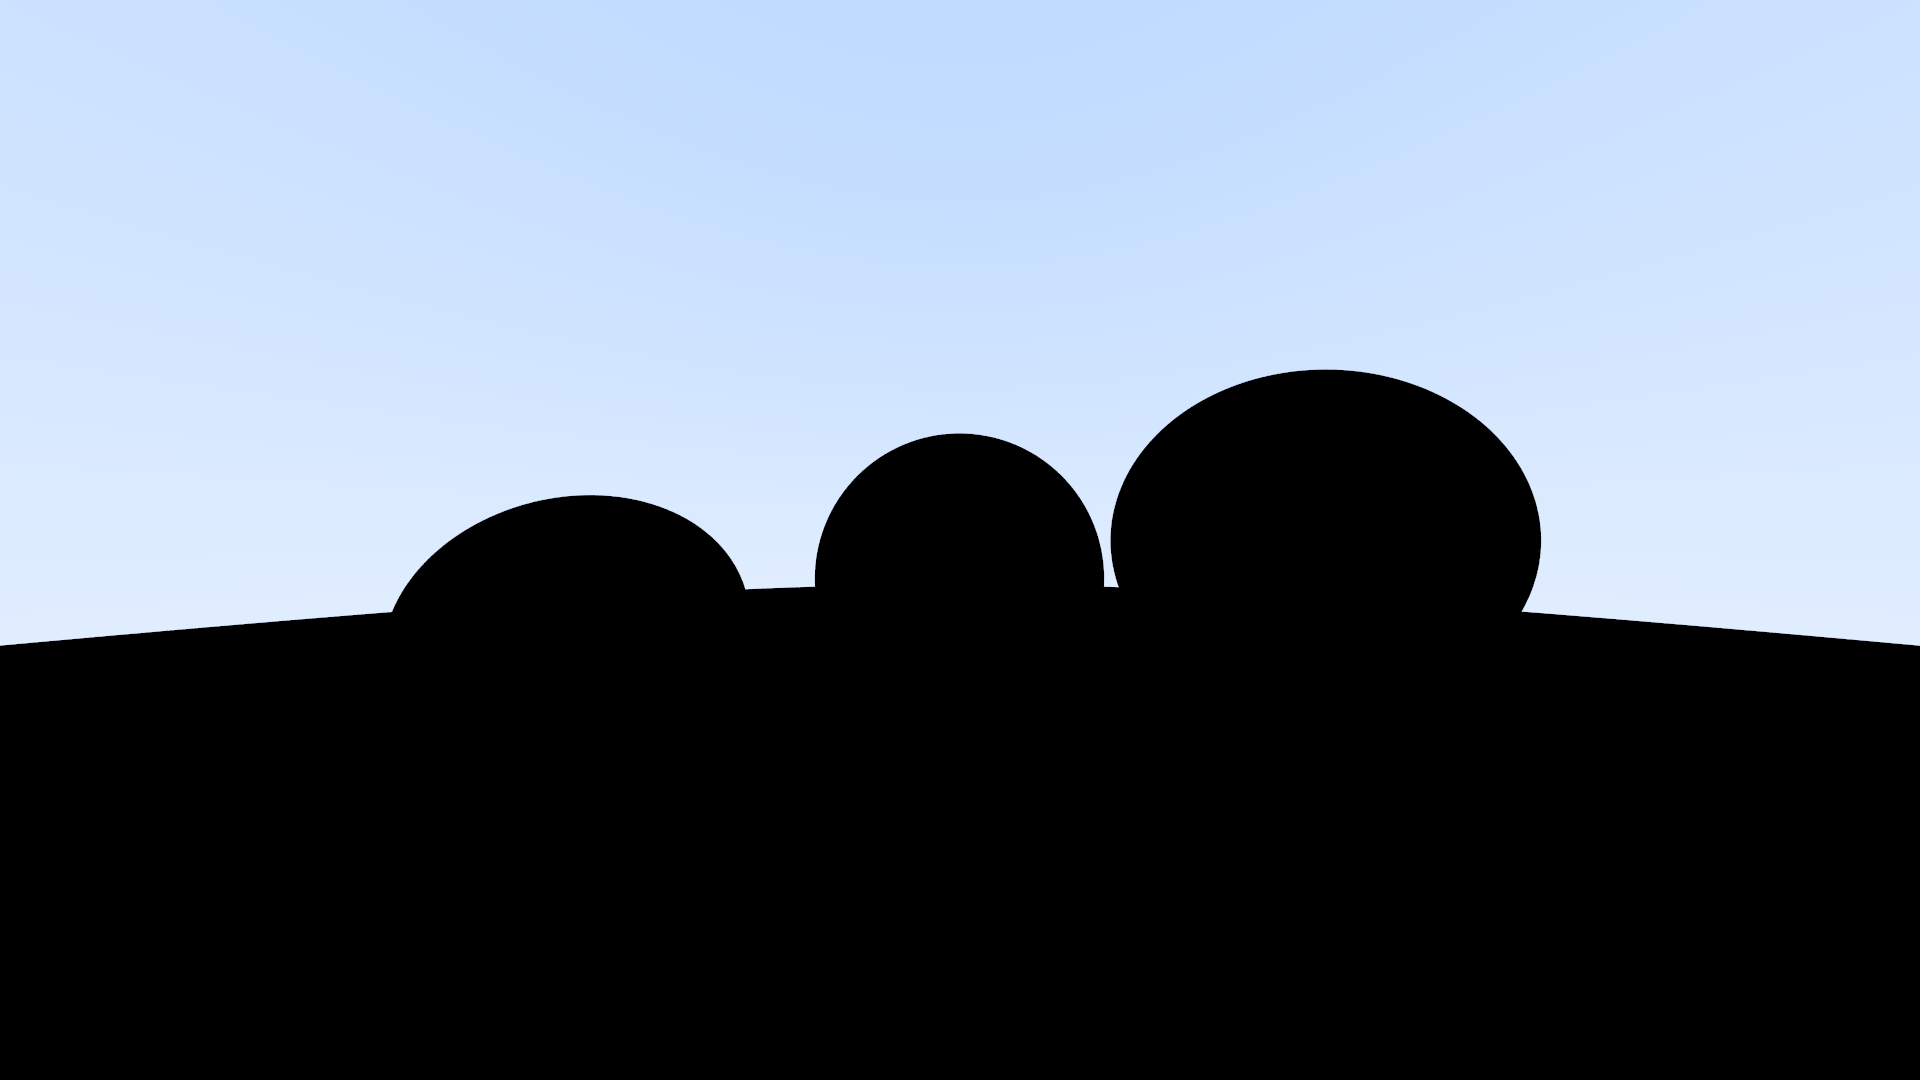
\includegraphics[width=0.3\linewidth]{image5}
			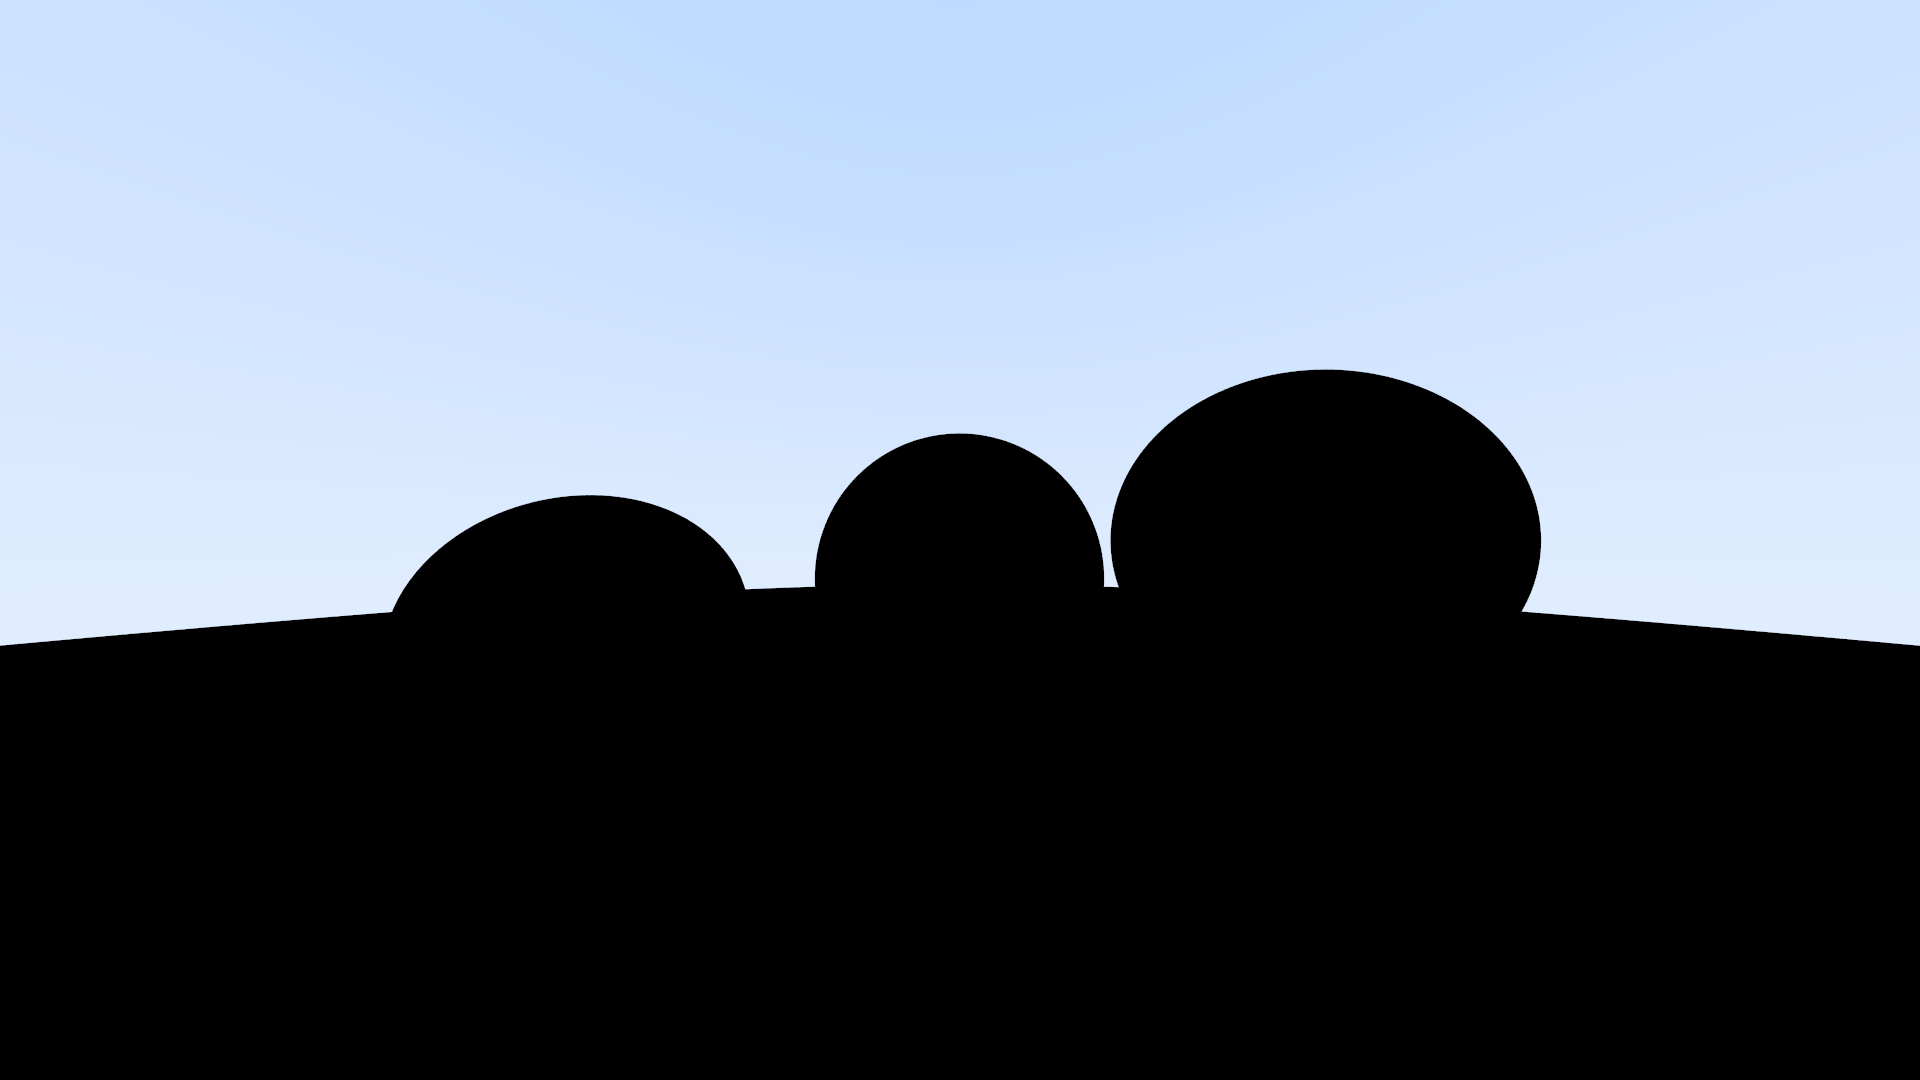
\includegraphics[width=0.3\linewidth]{image6}
			
\includegraphics[width=0.3\linewidth]{image7}
			\caption{Example images resulting from a \emph{max\textunderscore bounce\textunderscore depth} of 1}
			\label{fig:image567-black}
		\end{figure}
	
		In order no produce realistic renderings \emph{gamma correction} and a fix for \emph{shadow acne} are implemented in \emph{Camera} class in this step (following the tutorial).	
		
		\subsection{Diffuse}
		For a diffuse material just \emph{scatter} method must be overwritten. The implementation follows the tutorial \cite{Shirley2020RTW1}. Therefore, an attenuation color and a scattered ray have to be returned:
		\begin{enumerate}
			\item{The attenuation color is directly defined for a diffuse material as it’s \emph{albedo} color.}
			\item{The scattered ray is sent out in direction of the normal in the intersection point plus a random offset vector. This offset vector is a unit vector in a unit sphere. Basic concept of this procedure is to simulate true Lambertian reflection.}
		\end{enumerate}
	
		The corresponding code of the \emph{DiffuseMaterial} class representing diffuse materials is shown in \cref{lst:diffuse}.
		\begin{lstlisting}[caption={\emph{DiffuseMaterial} class}, language=Python, label=lst:diffuse]
class DiffuseMaterial(Material):
	# implementation of a diffuse material (inherits from Material)
	def __init__(self, albedo):
		self.albedo = albedo
	
	def scatter(self, ray, pos, norm, front_face):
		# returns scattered ray and color of material
		scatter_dir = norm + Vector.rand_in_unit_sphere().normalize()
		if scatter_dir.near_zero():
			scatter_dir = norm
		return Ray(pos, scatter_dir), self.albedo
		\end{lstlisting}
		
		Applying diffuse materials in \emph{scene5.py} on the 5 spheres shown in \cref{fig:image3} results in \cref{fig:image5}.
		
		\begin{figure}[h]
			\centering
			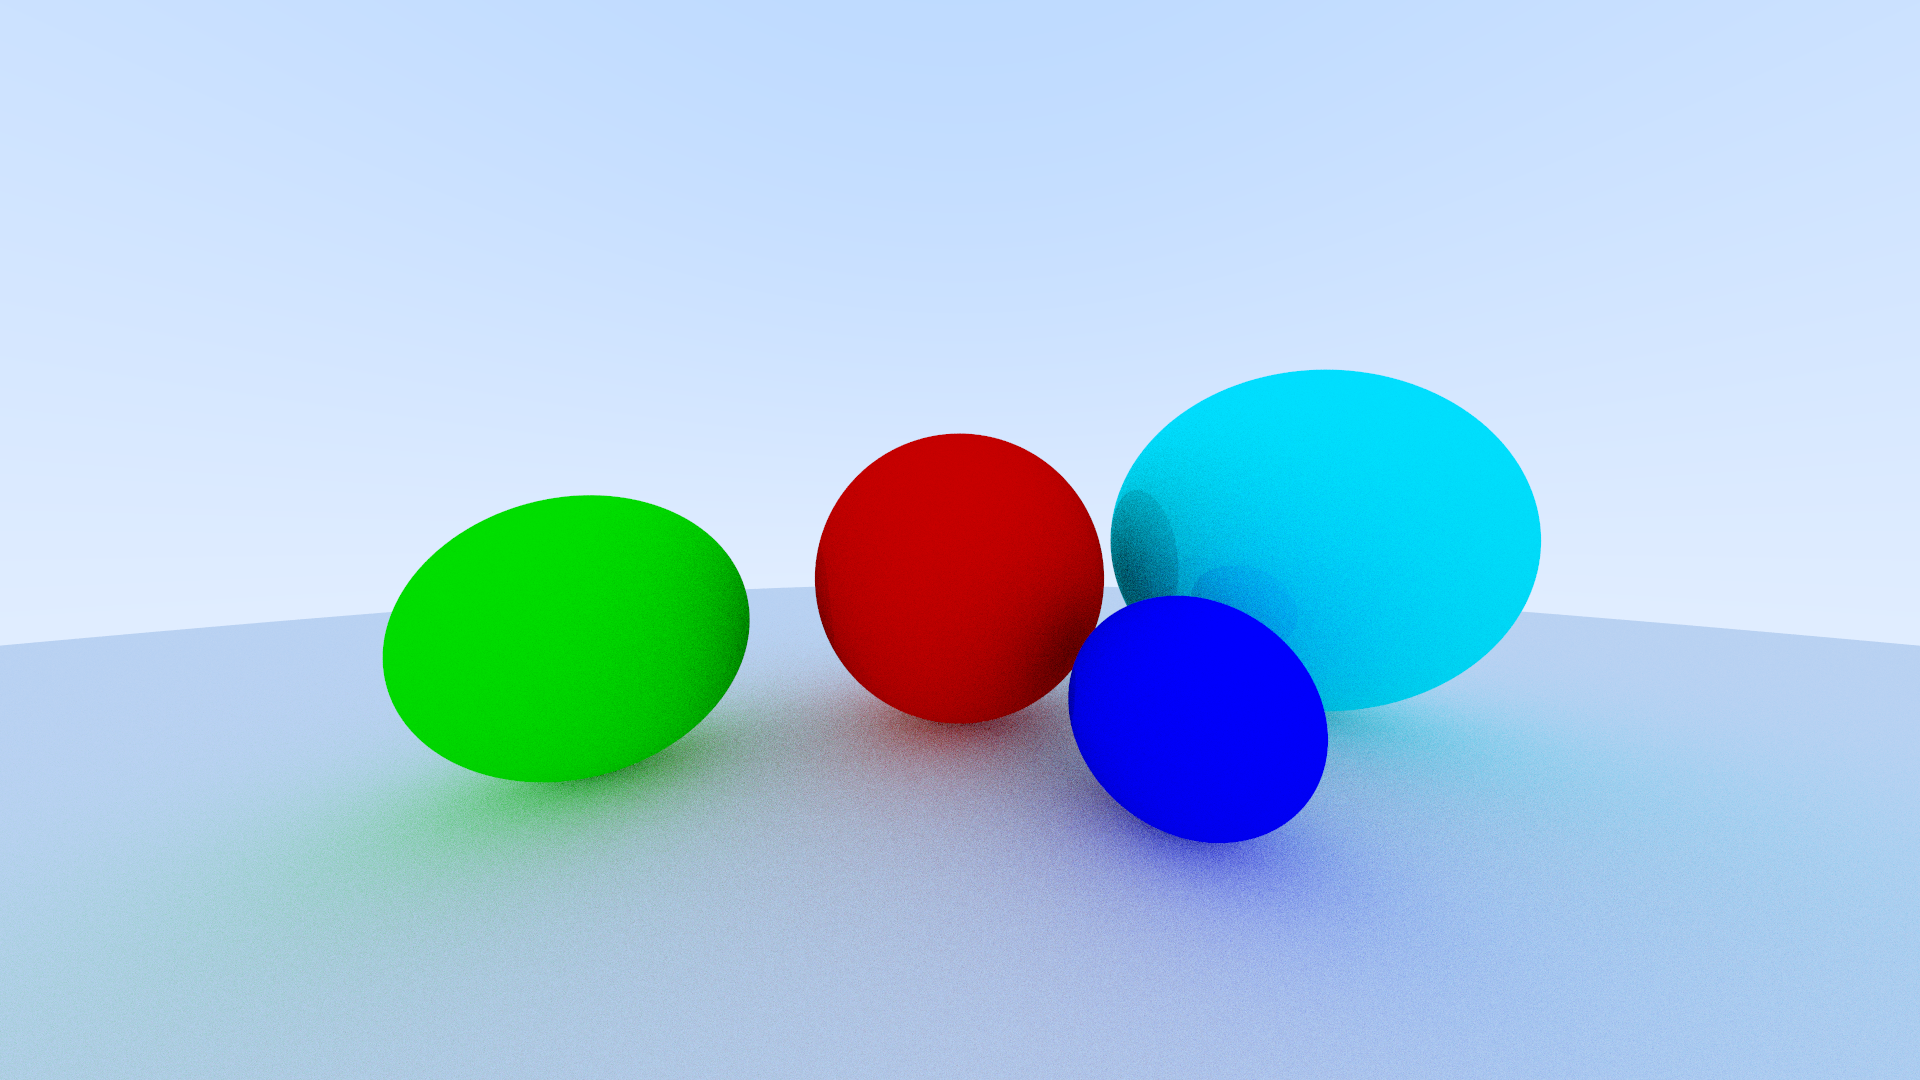
\includegraphics[width=0.9\linewidth]{image5-5}
			\caption{Scene of five spheres with diffuse material (\emph{max\textunderscore bounce\textunderscore depth} of 16)}
			\label{fig:image5}
		\end{figure}
		 
		\subsection{Specular}
		Specular material implemented in \emph{SpecularMaterial} class is similar to diffuse material. It also uses an albedo color for attenuation color. Main difference is the returned, scattered ray. On specular surfaces light is not randomly scattered but reflected. This is covered by law of reflection as described in lecture and tutorial and implemented in \emph{reflect(self, norm)} method called on the direction vector of the ray with the normal vector as the function parameter.
		
		\begin{lstlisting}[caption={Method for reflecting a vector on a normal vector}, language=Python, label=lst:reflect]
def reflect(self, norm):
	return self - norm * (self * norm) * 2
		\end{lstlisting}
		
		By adding 3 spheres to the last scenario in \emph{scene6.py} and applying different specular materials on them, the image in \cref{fig:image6} can be generated. One of those spheres is glossy as described in a bit more detail in \cref{sec:glossy}.
		
		\begin{figure}[h]
			\centering
			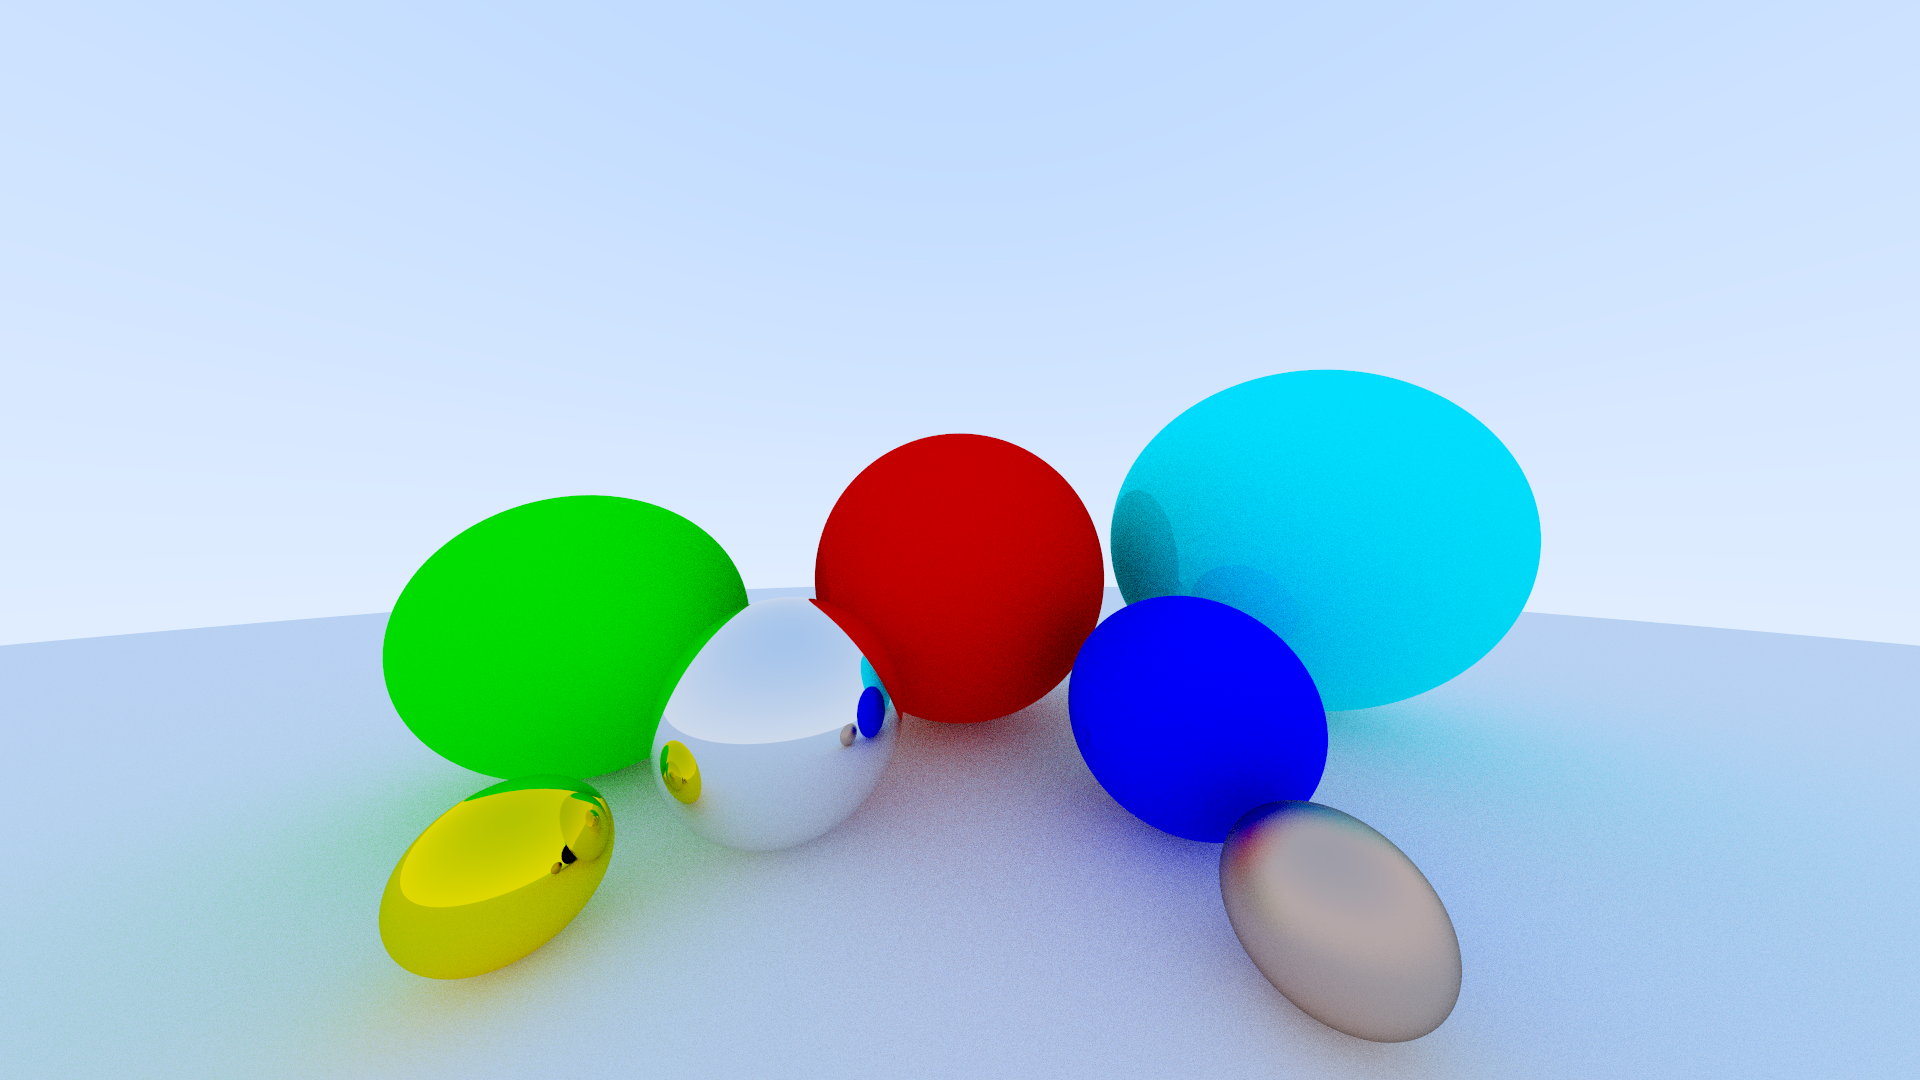
\includegraphics[width=0.9\linewidth]{image6-5}
			\caption{Scene of several spheres with diffuse and specular material (\emph{max\textunderscore bounce\textunderscore depth} of 16)}
			\label{fig:image6}
		\end{figure}
	
		\subsection{Glossy}
		\label{sec:glossy}
		In order to make a specular surface appear glossy a random offset is added to the direction of the reflected ray. This random offset is a vector within an unit sphere which is scaled by the so called \emph{fuzz} factor between 0 and 1. This factor is given to the material class by its constructor. This results in the default specular material for a \emph{fuzz} factor of 0 and more glossy specular materials for higher factors. If one of those scattered rays now do not point out of the sphere (no acute angle between normal and ray), the color black is returned (no light) and the recursion of \emph{ray\textunderscore color} is stopped.
	
		\subsection{Specular transmissive}
		For specular transmissive materials in addition to reflection the laws of refraction (Snell's law) must be taken into account for the calculation of the scattered rays direction and is therefore implemented as shown in \cref{lst:refract}. Basic concept is to use an \ac{ior} which is given to the constructor of the \emph{TransmissiveMaterial} class (no albedo color is used in this implementation). This \ac{ior} is a material specific constant and the reciprocal of the refraction ratio. With that information it's decided if reflection or refraction have to be used to determine the scattered ray's direction. In addition, as explained in the tutorial in \cite{Shirley2020RTW1} Schlick's approximation is applied to get more realistic results.
		
		\begin{lstlisting}[caption={Method for refracting a vector on a normal vector}, language=Python, label=lst:refract]
def refract(self, norm, cos_theta, eta_ratio):
	# cos_theta: already calculated cosinus of angle between vector and normal
	# eta_ratio: refraction ratio
	r_out_perp = (self + (norm * cos_theta)) * eta_ratio
	r_out_parallel = norm * -np.sqrt(np.abs(1-(r_out_perp*r_out_perp)))
	return r_out_perp + r_out_parallel			
		\end{lstlisting}
	
		With specular transmissive materials for example a glass ball can be simulated. But also hollow glass balls can be rendered easily by putting one sphere of smaller and negative radius within another. Such an hollow object and an additional transmissive sphere are added to the scene shown in the last section resulting in \emph{scene7.py} module and the image in \cref{fig:image7}. Because the hollow glass sphere is directly in front of the camera some interesting effects can be observed. For example some reflections within the sphere and distortions of objects, which are visible through and next to the sphere.
		
		\begin{figure}[h]
			\centering
			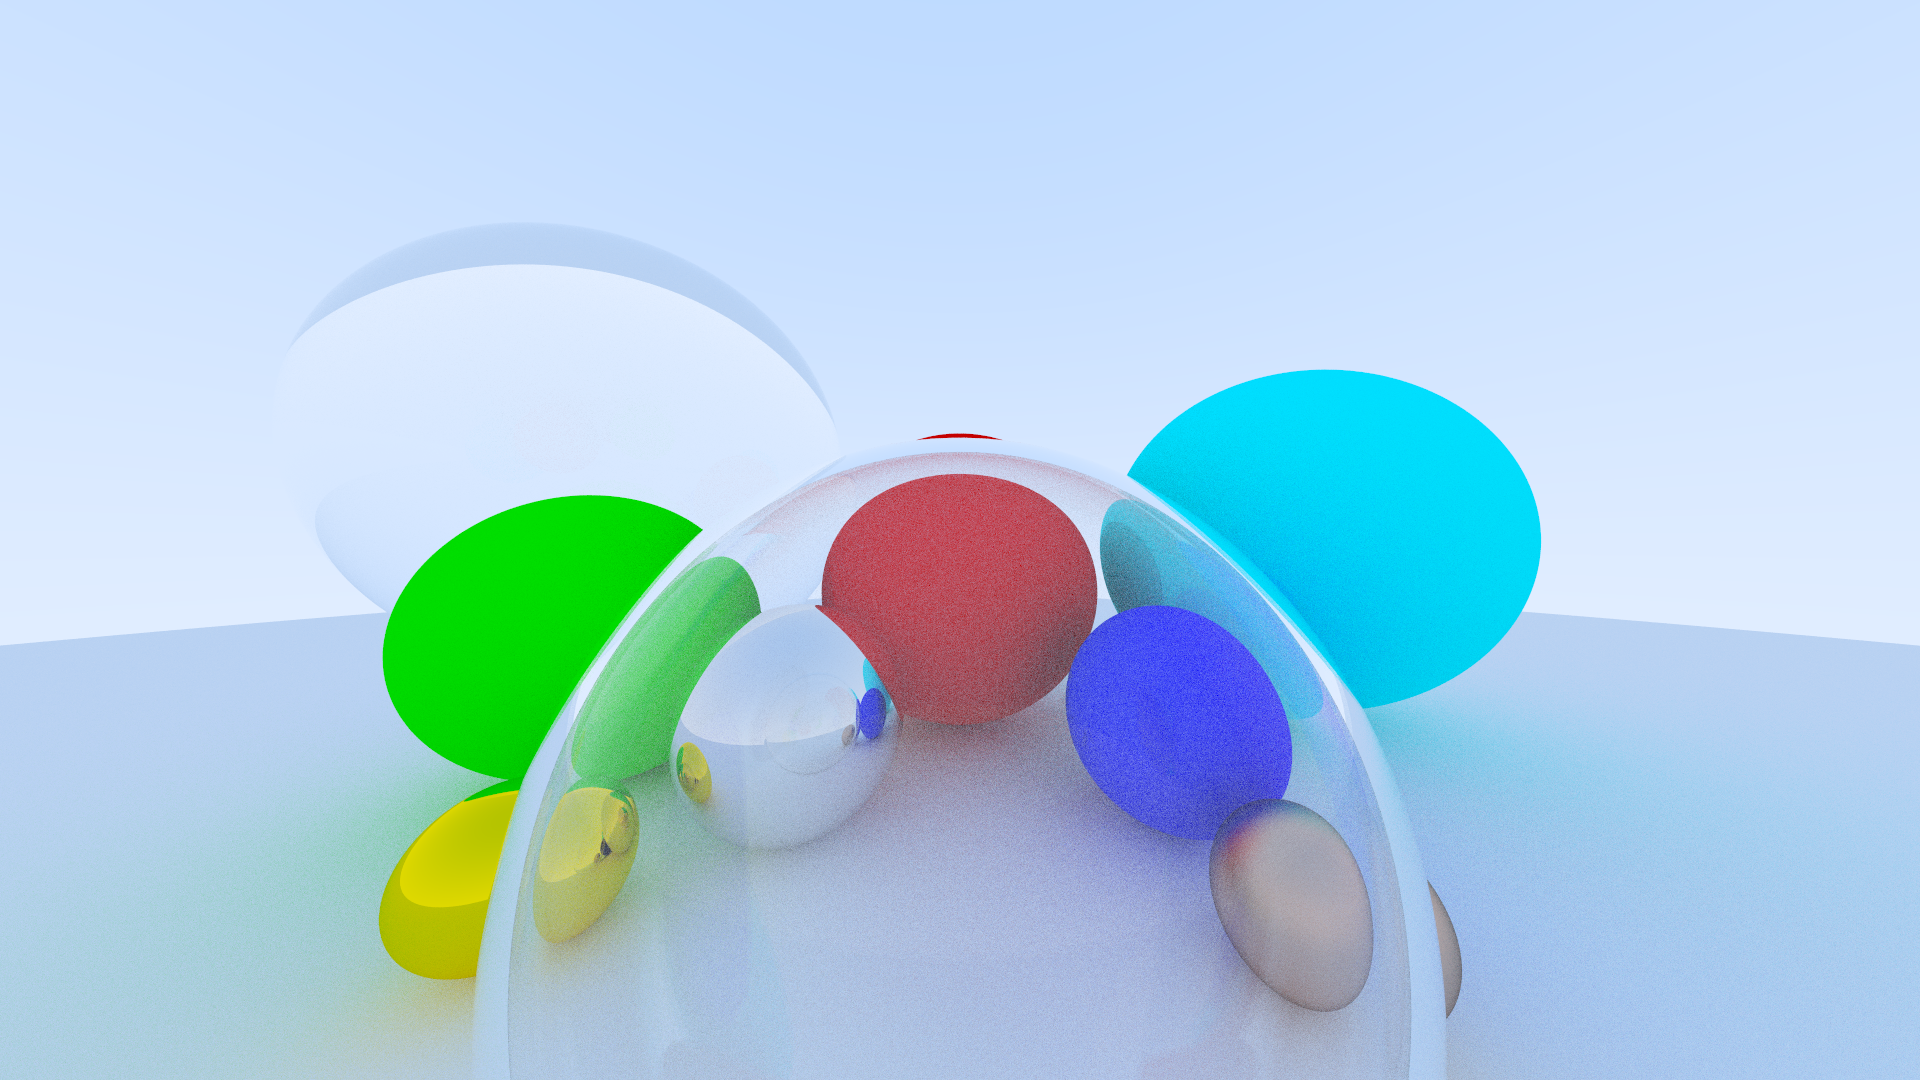
\includegraphics[width=0.9\linewidth]{image7-5}
			\caption{Scene of several spheres with diffuse, specular and specular transmissive material (\emph{max\textunderscore bounce\textunderscore depth} of 16)}
			\label{fig:image7}
		\end{figure}
				   
		\subsection{Emissive}
		Finally, in this implementation emissive materials are the only materials overwriting \emph{Material} class's \emph{emit()} method and also do not implement any kind of scattering. Main idea based on \cite{Shirley2020RTW2} is, to use a light \emph{color} and an \emph{intensity} given to the constructor of \emph{EmissiveMaterial} class and return the \emph{color} scaled with the \emph{intensity} in the \emph{emit()} method. This causes static color and therefore an unrealistic appearance of an emissive object itself, but it's an easy and valid approach for physical lights giving good results .
		\\
		While emissive objects also influence scenes with global illumination, their effects are quite more visible if no background lightning is used. Therefore, the \emph{Camera} class is extended by adding the possibility to change the color (gradient) of the background. By setting it to black and placing three spheres with emissive materials of different \emph{color} and an \emph{intensity} in \emph{scene8.py} the image in \cref{fig:image8} can be rendered. In order to generate high quality results and realistic lighting in addition to \emph{samples\textunderscore per\textunderscore pixel} also \emph{max\textunderscore bounce\textunderscore depth} is set to 64.
		
		\begin{figure}[h]
			\centering
			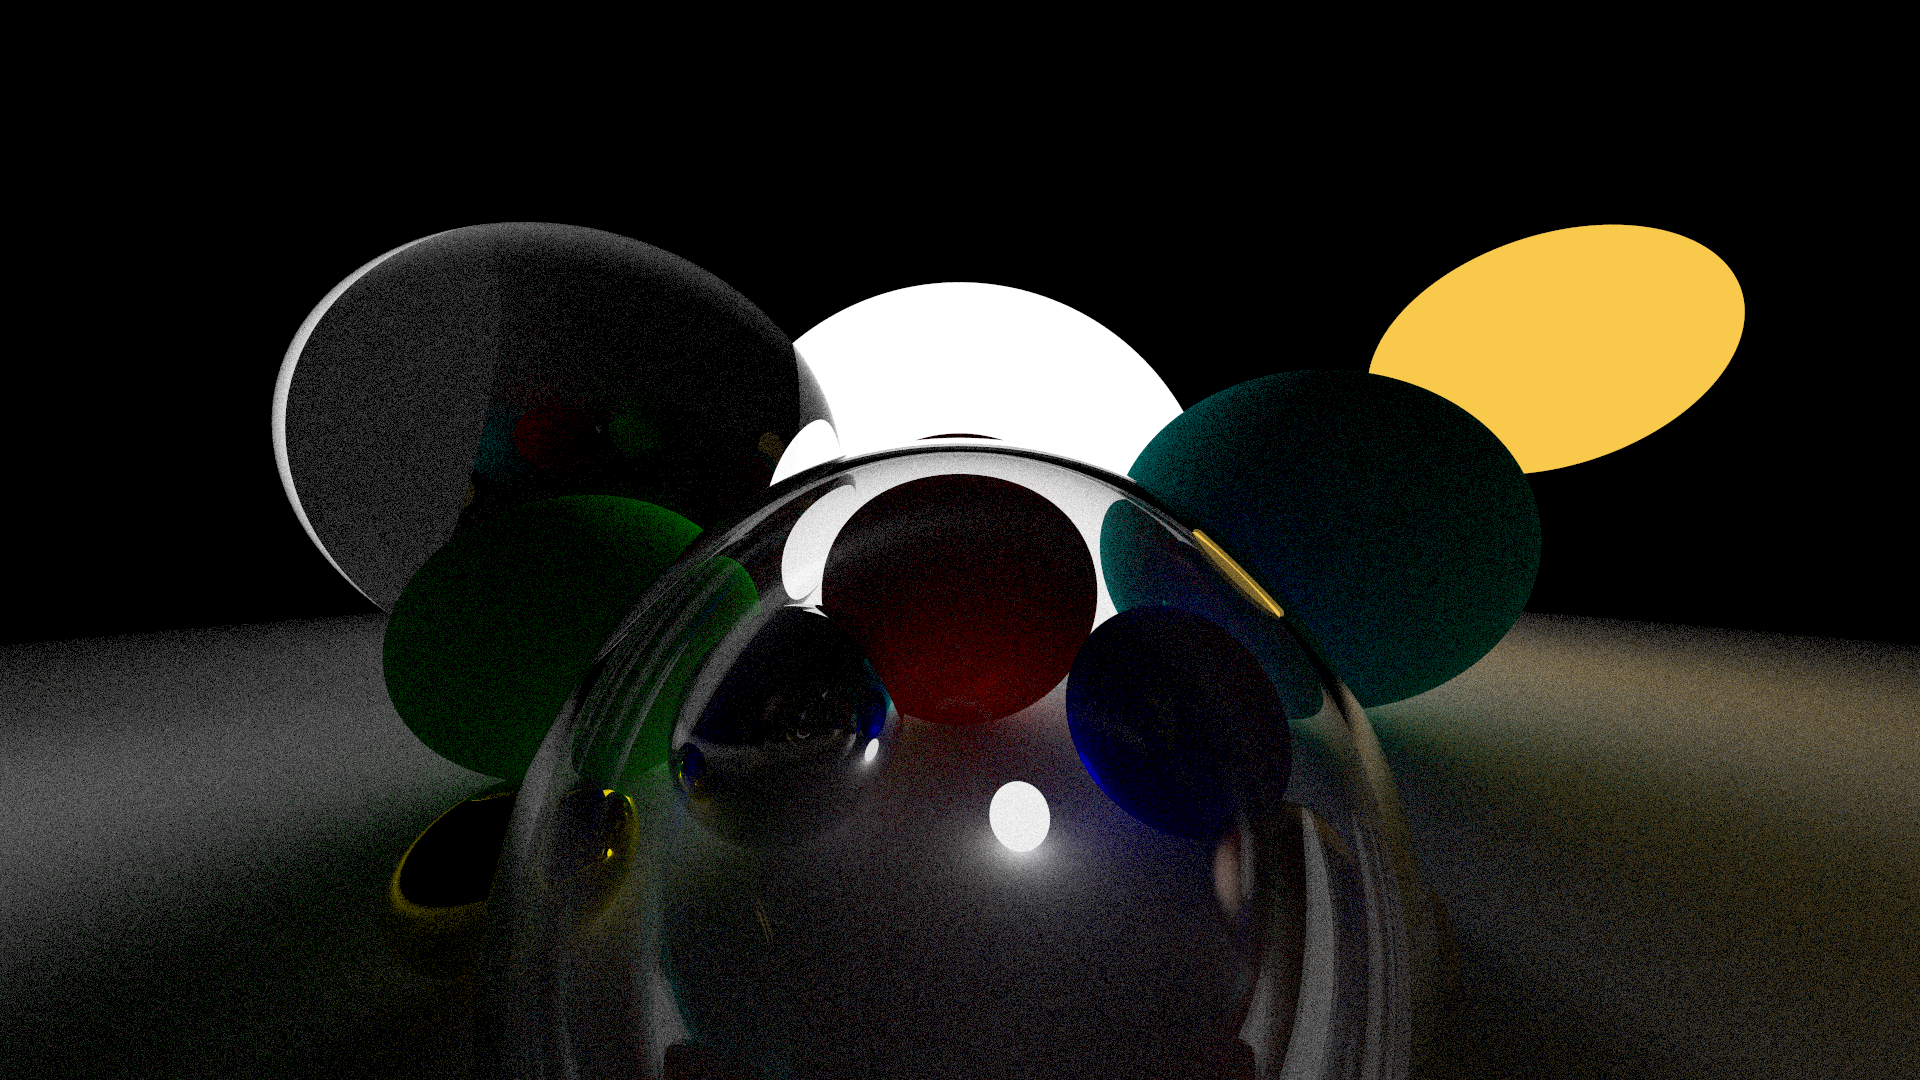
\includegraphics[width=0.9\linewidth]{image8}
			\caption{Scene of several spheres with diffuse, specular, specular transmissive and emissive material}
			\label{fig:image8}
		\end{figure}
		
	\section{Enhancing camera}
		The \emph{Camera} class introduced in \cref{sec:camera} provides already good results, but in order to get more realistic renderings two additional aspects are implemented as described in the following three subsections.
		
		\subsection{\ac{fov}}
		\label{sec:fov}
			To this point vertical and horizontal \ac{fov} are indirectly defined by the viewport size and the focal length parameter of the camera as shown in the tutorial. By introducing a parameter for vertical \ac{fov} as in \cite{Shirley2020RTW1} or for horizontal \ac{fov} as in this implementation (due to personal favor; like in most video games) the viewport size results from \ac{fov} and focal length.
			\\
			It's important to mention that for all rendered images the default horizontal \ac{fov} is set to $130^{\circ}$ (representing human horizontal \ac{fov}), while the \ac{fov} $\phi$ in \cite{Shirley2020RTW1} results from focal length $fl=1$, viewport height $vp_h=2$ and aspect ratio $ar=\label{key}16/9$ as shown in \cref{eq:fov}.
			
			\begin{equation}
				\label{eq:fov}
				\phi = 2\cdot arctan\left(\frac{vp_h\cdot ar}{2\cdot fl}\right) \approx 121,28^{\circ}
			\end{equation}
		 
			 Setting focal length always to one as in \cite{Shirley2020RTW1} is not a problem because all calculations are correctly implemented for this specific case, but for different focal length values wrong equations would be used to calculate the viewport. Therefore, if focal length as well as \ac{fov} are parameters of \emph{Camera} class, both values have to be used for correct viewport calculations with reordered \cref{eq:fov}. 
			 \\
			 Additionally, the trick for thin lens approximation explained in \cref{sec:depthoffield} is easier to implement, if focal length is used in all equations on default.
			
		\subsection{Positioning and orienting}
			A main feature of real cameras is that they can be moved around and the camera's angle can be changed. In order to provide this feature also with \emph{Camera} class the approach from the tutorial is used
			\\
			A \emph{lookfrom} vector defining the camera's position, a \emph{lookat} vector defining the point in space the camera is looking to and a up vector defining the up direction in camera's own coordinate system are given to the constructor of \emph{Camera} class. Using those three vectors an orthonormal basis of camera specific coordinate system can be calculated using cross products. This coordinate system is now used instead of forward, right and up vectors in world space coordinates.
			\\
			By adding five more spheres to the current scene and changing camera's position and orientation in \emph{scene9.py} it's possible to render images from interesting perspectives as shown in \cref{fig:image9}.
			
			\begin{figure}[h]
				\centering
				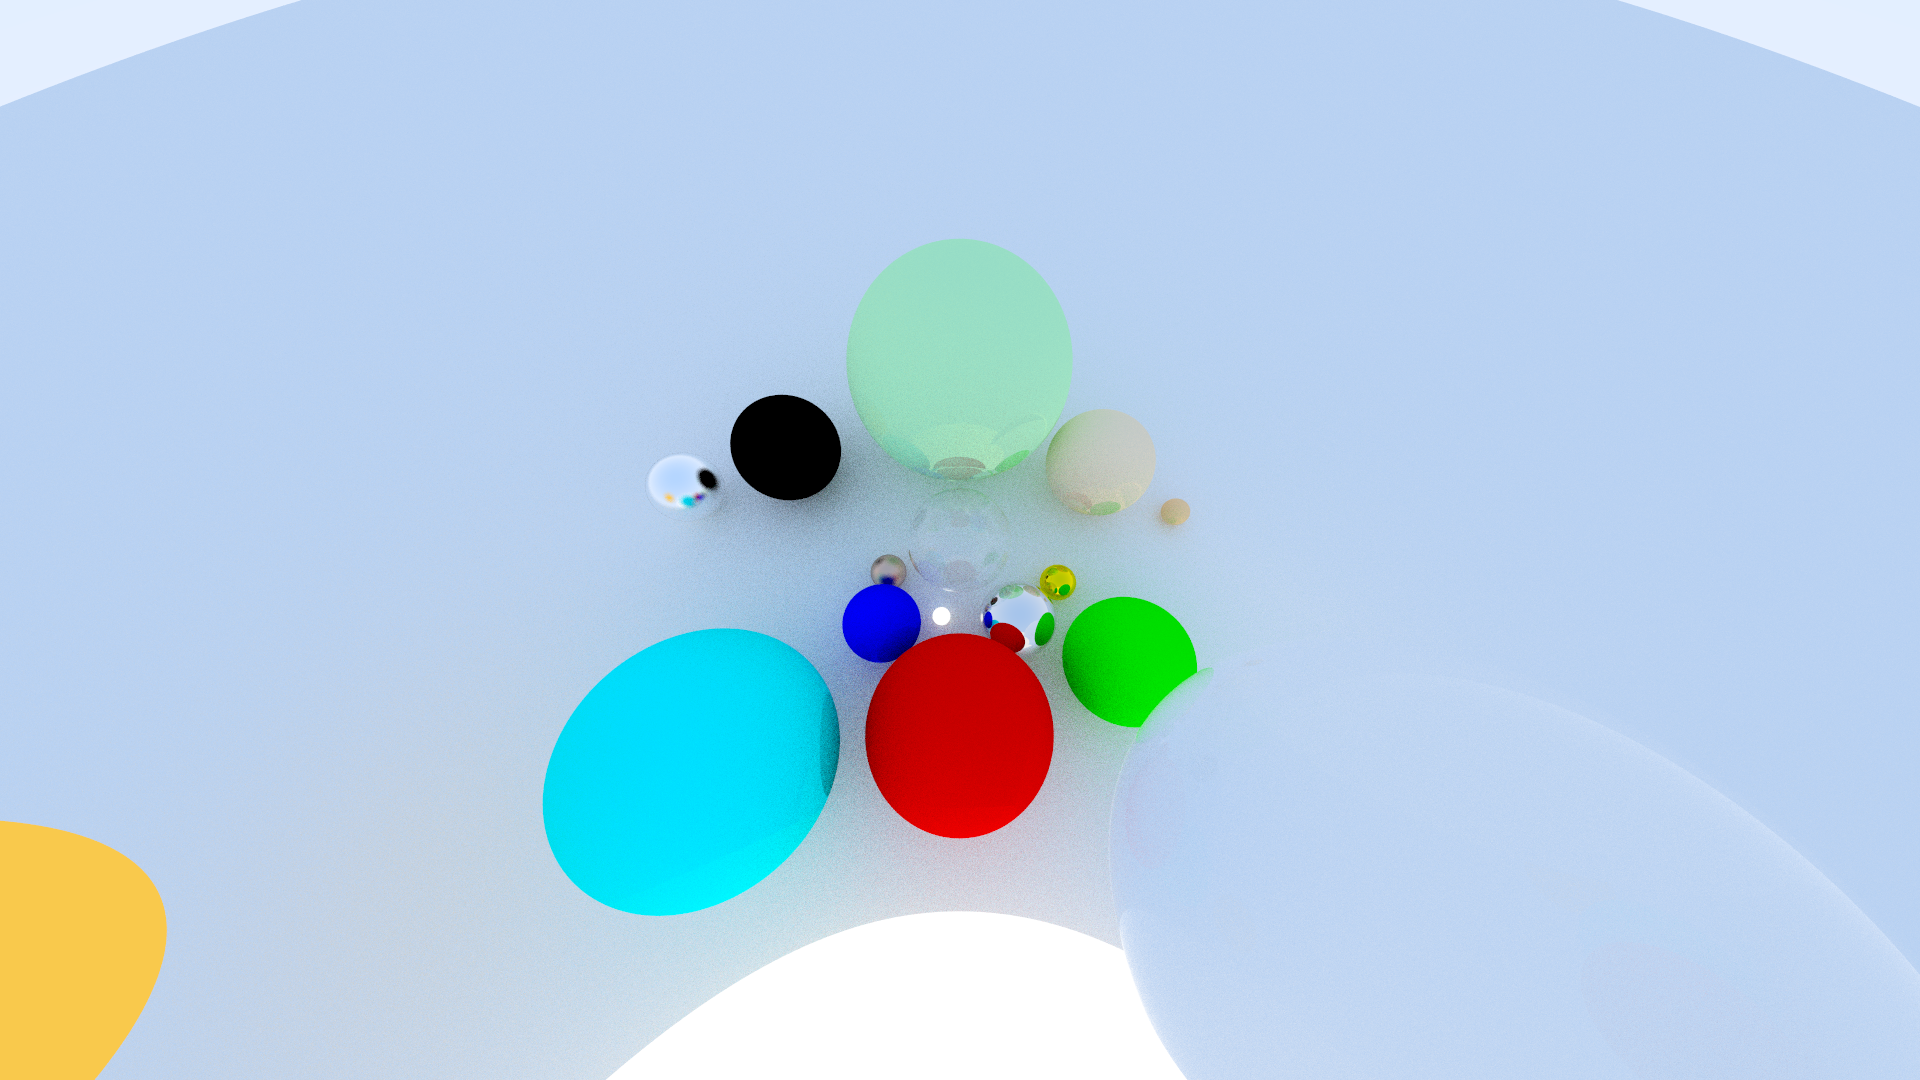
\includegraphics[width=0.30\linewidth]{image9}
				\includegraphics[width=0.30\linewidth]{image9-1}
				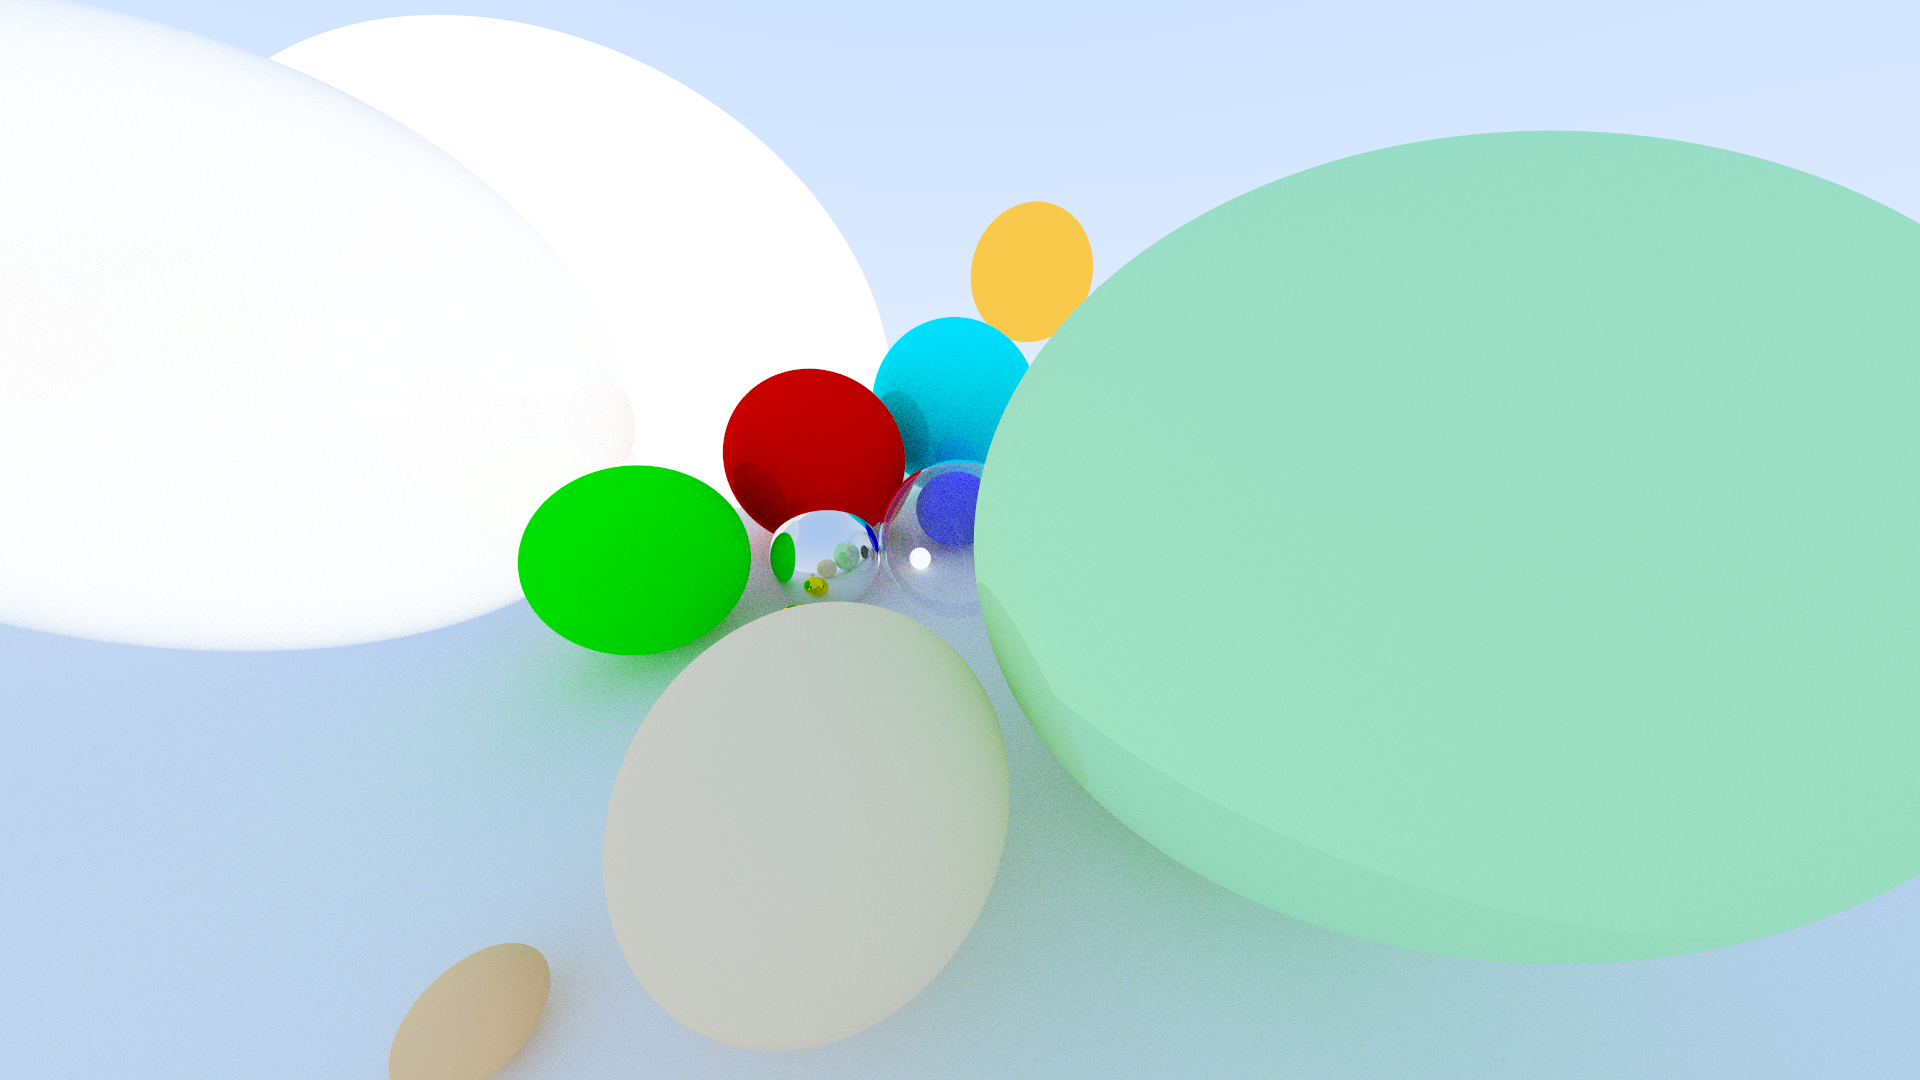
\includegraphics[width=0.30\linewidth]{image9-2}
				\caption{Scene of several spheres with various materials rendered from different perspectives}
				\label{fig:image9}
			\end{figure}			
			
		\subsection{Depth of field}
		\label{sec:depthoffield}
			Another effect in real photography is depth of field. Due to lenses and apertures used in real cameras only objects in a limited range around a certain distance are perfectly sharp. While it's also an advantage of rendering to be able to generate globally sharp images, often depth of field is a desired effect. 
			\\
			In order to simulate it there are basically two different approaches of approximation:
			
			\begin{enumerate}
				\item{\emph{Thick lens approximation}}
				\item{\emph{Thin lens approximation}}  
			\end{enumerate}
			\emph{Thick lens approximation} is simulating a real lens of certain thickness (scaled up to complex structures of multiple lenses). 
			\\
			\emph{Thin lens approximation} used in this implementation inspired by \cite{Shirley2020RTW1} avoids those complex and intense calculations by simulating the lens with random offsets of camera center and a clever usage of focal length.
			\\
			Having a last closer look on \cref{lst:getray} shows the implementation of random offsets of the camera's center. All rays are not longer sent out only from the center but a random offset within an unit disc (radius equals to aperture radius) is added to the center position. Only objects which are located on the image plane will be rendered as before, others will be blurred. Finally, the last step of the \emph{Thin lens approximation} is to set focal length to the desired depth of field to grant the expected behavior.
		
			\begin{lstlisting}[caption={Method to generate a ray for given pixel coordinates using antialisaing and thin lens approximation}, language=Python, label=lst:getray]
def get_ray(self, x, y, antialiasing):
	# antialiasing offset
	rand_offset_x, rand_offset_y = 0, 0
	# depth of field offset (lens)
	lens_offset = Vector.rand_in_unit_disc() * self.lens_radius
	position_offset = self.u * lens_offset.x + self.v * lens_offset.y
	
	if antialiasing:
		rand_offset_x = np.random.uniform(0, 1)
		rand_offset_y = np.random.uniform(0, 1)
	
	return Ray(self.position + position_offset, self.lower_left_corner 
		+ self.horizontal * (x + rand_offset_x) / (self.image_width - 1) 
		+ self.vertical * (y + rand_offset_y) / (self.image_height - 1) 
		- self.position - position_offset)
			\end{lstlisting}
	
	\section{Conclusion}
	
	\clearpage
	\printbibliography[heading=bibintoc].
		
\end{document}
